% Options for packages loaded elsewhere
\PassOptionsToPackage{unicode}{hyperref}
\PassOptionsToPackage{hyphens}{url}
\PassOptionsToPackage{dvipsnames,svgnames*,x11names*}{xcolor}
%
\documentclass[
  11pt,
]{article}
\usepackage{lmodern}
\usepackage{amssymb,amsmath}
\usepackage{ifxetex,ifluatex}
\ifnum 0\ifxetex 1\fi\ifluatex 1\fi=0 % if pdftex
  \usepackage[T1]{fontenc}
  \usepackage[utf8]{inputenc}
  \usepackage{textcomp} % provide euro and other symbols
\else % if luatex or xetex
  \usepackage{unicode-math}
  \defaultfontfeatures{Scale=MatchLowercase}
  \defaultfontfeatures[\rmfamily]{Ligatures=TeX,Scale=1}
\fi
% Use upquote if available, for straight quotes in verbatim environments
\IfFileExists{upquote.sty}{\usepackage{upquote}}{}
\IfFileExists{microtype.sty}{% use microtype if available
  \usepackage[]{microtype}
  \UseMicrotypeSet[protrusion]{basicmath} % disable protrusion for tt fonts
}{}
\makeatletter
\@ifundefined{KOMAClassName}{% if non-KOMA class
  \IfFileExists{parskip.sty}{%
    \usepackage{parskip}
  }{% else
    \setlength{\parindent}{0pt}
    \setlength{\parskip}{6pt plus 2pt minus 1pt}}
}{% if KOMA class
  \KOMAoptions{parskip=half}}
\makeatother
\usepackage{xcolor}
\IfFileExists{xurl.sty}{\usepackage{xurl}}{} % add URL line breaks if available
\IfFileExists{bookmark.sty}{\usepackage{bookmark}}{\usepackage{hyperref}}
\hypersetup{
  colorlinks=true,
  linkcolor=Maroon,
  filecolor=Maroon,
  citecolor=Blue,
  urlcolor=blue,
  pdfcreator={LaTeX via pandoc}}
\urlstyle{same} % disable monospaced font for URLs
\usepackage[margin=1in]{geometry}
\usepackage{graphicx,grffile}
\makeatletter
\def\maxwidth{\ifdim\Gin@nat@width>\linewidth\linewidth\else\Gin@nat@width\fi}
\def\maxheight{\ifdim\Gin@nat@height>\textheight\textheight\else\Gin@nat@height\fi}
\makeatother
% Scale images if necessary, so that they will not overflow the page
% margins by default, and it is still possible to overwrite the defaults
% using explicit options in \includegraphics[width, height, ...]{}
\setkeys{Gin}{width=\maxwidth,height=\maxheight,keepaspectratio}
% Set default figure placement to htbp
\makeatletter
\def\fps@figure{htbp}
\makeatother
\setlength{\emergencystretch}{3em} % prevent overfull lines
\providecommand{\tightlist}{%
  \setlength{\itemsep}{0pt}\setlength{\parskip}{0pt}}
\setcounter{secnumdepth}{5}
\usepackage{setspace}
\usepackage{float}
\usepackage{mathtools}
\usepackage{natbib}
\usepackage[linesnumbered,ruled,vlined]{algorithm2e}
\setcitestyle{numbers,square,comma}
\usepackage{verbatim}
\usepackage{amsthm}
\usepackage{comment}
\usepackage[]{natbib}
\bibliographystyle{plainnat}

\author{}
\date{\vspace{-2.5em}}

\begin{document}


\pagenumbering{gobble}

%\begin{titlepage}
\begin{center}
\LARGE{\textbf{Community Detection Methods for the Generalized Random Dot Product Graph Model}}\\
\vspace*{2\baselineskip}
\normalsize{A dissertation proposal submitted in partial satisfaction of the requirements for the degree of \\}
Doctor of Philosophy \\
in \\
Statistical Science \\
\vspace*{2\baselineskip}
\Large{John Koo}\\
\vspace*{3\baselineskip}
\Large{\textbf{Research Committee Members}}\\
Dr. Michael Trosset \\
Dr. Minh Tang \\
Dr. Julia Fukuyama \\
Dr. Roni Khardon \\
Dr. Fangzheng Xie \\
\vspace*{3\baselineskip}
June 2, 2021 \\
\vspace*{1\baselineskip}
Department of Statistics \\
Indiana University \\
Bloomington, Indiana \\
\end{center}
% \end{titlepage}

\hypersetup{linkcolor = black}
\newpage
\pagenumbering{roman}
\tableofcontents
\addcontentsline{toc}{section}{\contentsname}

\newpage

\begin{center}
\LARGE{Abstract}
\end{center}

\vspace*{2\baselineskip}

\normalsize

Graph and network data, in which samples are represented not as a collection of feature vectors but as relationships between pairs of observations, are increasingly widespread in various fields ranging from sociology to computer vision. One common goal of analyzing graph data is community detection or graph clustering, in which the graph is partitioned into disconnected subgraphs in an unsupervised yet meaningful manner (e.g., by optimizing an objective function or recovering unobserved labels). Because traditional clustering techniques were developed for data that can be represented as vectors, they cannot be applied directly to graphs. In this research, we investigate the use of a family of spectral decomposition based approaches for community detection in block models (random graph models with inherent community structure), first by demonstrating how under the Generalized Random Dot Product Graph framework, all graphs generated by block models can be represented as feature vectors, then applying clustering methods for these feature vector representations, and finally deriving the asymptotic properties of these methods. 

\newpage
\pagenumbering{arabic}
\hypersetup{linkcolor = blue}

\newcommand{\diag}{\text{diag}}
\newcommand{\tr}{\text{Tr}}
\newcommand{\blockdiag}{\text{blockdiag}}
\newcommand{\indep}{\stackrel{\text{ind}}{\sim}}
\newcommand{\iid}{\stackrel{\text{iid}}{\sim}}
\newcommand{\Bernoulli}{\text{Bernoulli}}
\newcommand{\Betadist}{\text{Beta}}
\newcommand{\BG}{\text{BernoulliGraph}}
\newcommand{\Cat}{\text{Categorical}}
\newtheorem{definition}{Definition}
\newtheorem{theorem}{Theorem}
\newtheorem{lemma}{Lemma}
\theoremstyle{remark}
\newtheorem*{remark}{Remark}
\theoremstyle{example}
\newtheorem*{example}{Example}

\hypertarget{introduction}{%
\section{Introduction}\label{introduction}}

\hypertarget{research-goal}{%
\subsection{Research Goal}\label{research-goal}}

Graph and network data have become increasingly widespread in various
fields including sociology, neuroscience, biostatistics, and computer
science. This has resulted in various challenges for researchers who
rely on traditional statistical and machine learning methods, many of
which are incompatible with graph data and instead require the data to
exist as feature vectors in Euclidean space. This includes graph
clustering and community detection, which are often the goal of data
analysis on graphs and networks. Common clustering methods typically
involve calculating some central or representative point for each
cluster around which the data belonging to that cluster lie (e.g.,
Lloyd's algorithm for \(K\)-means clustering \cite{1056489}, Gaussian
Mixture Models \cite{doi:10.1198/016214502760047131}). Because these
methods involve computing summary statistics within each cluster, such
as the sample average, they cannot be applied directly to graphs,
necessitating methods for transforming the graph data into feature
vectors if they are to be used.

One family of methods for unifying graph community detection with
traditional clustering techniques is Spectral Clustering
\cite{DBLP:journals/corr/abs-0711-0189}, which involves embedding the
graph into Euclidean space, followed by applying a popular clustering
algorithm such as \(K\)-means clustering. The Random Dot Product Graph
(RDPG) \cite{10.1007/978-3-540-77004-6_11} and Generalized Random Dot
Product Graph (GRDPG) \cite{rubindelanchy2017statistical} models take
this further by explicitly constructing generative models for graphs via
latent vectors in Euclidean space. In such a model, each vertex has a
corresponding vector in latent space, and the edge probabilities between
pairs of vertices are computed by operations on the corresponding pairs
of latent vectors. A community detection algorithm motivated by this may
involve learning the latent positions given an observed graph and then
learning the community labels given the latent positions.

The aim of our research is to develop consistent community detection
techniques under the RDPG and GRDPG frameworks. First, we explore
existing generative graph models with underlying community structures
(Block Models) that can be inferred by connecting these models to the
RDPG or GRDPG. In particular, we use the connection between the
Popularity Adjusted Block Model \cite{307cbeb9b1be48299388437423d94bf1}
and the GRDPG to motivate two community detection methods. Then we
explore other latent structures or mixture distributions in the latent
space that induce graphs for which consistent community detection is
possible.

\hypertarget{notation}{%
\subsection{Notation}\label{notation}}

Let \(G = (V, E)\) be an undirected, unweighted graph with no self-loops
and \(n\) vertices. Denote \(A \in \{0, 1\}^{n \times n}\) as the
adjacency matrix of \(G\) such that \(A_{ij} = 1\) if there exists an
edge between vertices \(i\) and \(j\) and \(A_{ij} = 0\) otherwise.
Because \(G\) is symmetric and contains no self-loops,
\(A_{ij} = A_{ji}\) and \(A_{ii} = 0\) for \(i, j \in [n]\). We further
restrict our analyses to independent Bernoulli graphs. Let
\(P \in [0, 1]^{n \times n}\) be a symmetric matrix of edge
probabilities. Graph \(G\) is sampled from \(P\) by drawing
\(A_{ij} \stackrel{\text{ind}}{\sim}\text{Bernoulli}(P_{ij})\) for each
\(1 \leq i < j \leq n\) (\(A_{ji} = A_{ij}\) and \(A_{ii} = 0\)). We
denote \(A \sim \text{BernoulliGraph}(P)\) as graph with adjacency
matrix \(A\) sampled from edge probability matrix \(P\) in this manner.
If each vertex has a hidden label in \([K]\), they are denoted as
\(z_1, ..., z_n\). Finally, we denote
\(X = \begin{bmatrix} x_1 & \cdots & x_n \end{bmatrix}^\top \in \mathbb{R}^{n \times d}\)
as the sample \(x_1, ..., x_n \in \mathbb{R}^d\).

\hypertarget{preliminaries}{%
\section{Preliminaries}\label{preliminaries}}

\hypertarget{block-models}{%
\subsection{Block Models}\label{block-models}}

Generative models for independent Bernoulli graphs involve defining the
edge probability matrix \(P\) whose \(ij\)\textsuperscript{th} entry is
the probability of an edge between vertices \(i\) and \(j\) for each
\(i, j \in [n]\). In order to motivate community detection methods, we
restrict the generative model such that for each pair of vertices
\((i, j)\), the probability of an edge between the vertices \(P_{ij}\)
depends in some way on their labels \(z_i\) and \(z_j\). Such models are
called Block Models.

One type of Block Model is the Stochastic Block Model (SBM)
\cite{doi:10.1080/0022250X.1971.9989788}: Given \(K\) communities and
each vertex belonging to one of the \(K\) communities, the SBM restricts
\(P\) to \(K (K + 1) / 2\) unique entries such that
\(P_{ij} = p_{z_i z_j}\) where \(p_{kl} = p_{lk}\) is the probability of
an edge between each vertex in community \(k\) to each vertex in
community \(l\). The homogeneous SBM further restricts \(P\) to two
unique entries: \(P_{ij} = p\) if \(z_i = z_j\) and \(P_{ij} = q\)
otherwise. Several generalizations of the SBM have been introduced
since, including the Degree Corrected Block Model (DCBM)
\cite{Karrer_2011} and the Popularity Adjusted Block Model (PABM)
\cite{307cbeb9b1be48299388437423d94bf1}. Like the SBM, these models
involve imposing some restriction on \(P\) based on community labels
(and possibly other factors).

\hypertarget{generalized-random-dot-product-graphs}{%
\subsection{(Generalized) Random Dot Product
Graphs}\label{generalized-random-dot-product-graphs}}

Like the SBM, DCBM, and PABM, the RDPG and GRDPG are generative models
for graphs involving an edge probability matrix \(P\). The RDPG starts
with points in latent space \(X \in \mathcal{X} \subset \mathbb{R}^d\)
for \(\mathcal{X} = \{x, y \in \mathbb{R}^d : x^\top y \in [0, 1]\}\).
\(P\) is then constructed as \(P = X X^\top\), and
\(A \sim \text{BernoulliGraph}(P)\). We provide a more formal definition
of the RDPG and GRDPG as follows:

\begin{definition}[(Generalized) Random Dot Product Graph]
Let $X \in \mathbb{R}^{n \times d}$ be a collection of $n$ points in $\mathcal{X} \subset \mathbb{R}^d$ where $\mathcal{X} = \{x, y \in \mathbb{R}^d : x^\top y \in [0, 1]\}$. $G = (V, E)$ is a Random Dot Product Graph if its adjacency matrix is drawn as $A \sim \text{BernoulliGraph}(X X^\top)$. 

If on the other hand, $\mathcal{X} = \{x, y \in \mathbb{R}^{p+q} : x^\top I_{p, q} y \in [0, 1]\}$ and $A \sim \text{BernoulliGraph}(X I_{p, q} X^\top)$ for $I_{p, q} = \text{blockdiag}(I_p, -I_q)$ and $p + q = d$, then $A$ is the adjacency matrix of a Generalized Random Dot Product Graph. These are denoted by $A \sim \text{RDPG}(X)$ and $A \sim \text{GRDPG}_{p, q}(X)$ respectively.

In addition, let $F$ be a probability distribution with support $\mathcal{X}$, and $X_1, ..., X_n \stackrel{iid}{\sim} F$ with $X = \begin{bmatrix} X_1 & \cdots & X_n \end{bmatrix}^\top$. If $A$ is drawn from $X$ as before, then $(A, X) \sim \text{RDPG}(F, n)$ or $(A, X) \sim \text{GRDPG}_{p, q}(F, n)$. 
\end{definition}

The structure of the RDPG and GRDPG provides a straightforward method
for recovery of the latent positions via spectral decomposition.

\begin{definition}[Adjacency Spectral Embedding]
Let $A \sim \text{RDPG}(X)$ for $X \in \mathcal{X} \subset \mathbb{R}^{n \times d}$. Let $A \approx V \Lambda V^\top$ be the approximate spectral decomposition of $A$ corresponding to the $d$ largest eigenvalues and their corresponding eigenvectors. Then the rows of $V \Lambda^{1/2}$ are the scaled Adjacency Spectral Embedding (ASE) of $A$, and the rows of $V$ are the unscaled ASE of $A$. 

If $A \sim \text{GRDPG}_{p, q}(X)$, then let $A \approx V \Lambda V^\top$ be the approximate spectral decomposition of $A$ corresponding to the $p$ most positive and $q$ most negative eigenvalues of $A$ and their corresponding eigenvectors. Then the rows of $V |\Lambda|^{1/2}$ and $V$ are the scaled and unscaled ASE of $A$ respectively.
\end{definition}

\citet{athreya2017statistical} showed that under mild conditions, if
\((A_n, X_n) \sim \text{RDPG}(F, n)\) and \(\hat{X}_n\) is the scaled
ASE of \(A_n\), for some sequence of orthogonal matrices \(\{W_n\}\),

\begin{equation}
\max_i \|(\hat{X}_n)_i - W_n (X_n)_i \| \stackrel{a.s.}{\to} 0
\end{equation}

Similarly, \citet{rubindelanchy2017statistical} showed that for
\((A_n, X_n) \sim \text{GRDPG}_{p, q}(F, n)\),

\begin{equation}
\max_i \|(\hat{X}_n)_i - Q_n (X_n)_i \| \stackrel{a.s.}{\to} 0
\end{equation}

where \(\{Q_n\}\) is a sequence of matrices in \(\mathbb{O}(p, q)\), the
indefinite orthogonal group of order \(p, q\).

It is straightforward to show that all Bernoulli graphs with positive
semidefinite \(P\) are special cases of the RDPG, which is a special
case of the GRDPG, and all Bernoulli Graphs generated by \(P\)
regardless of positive semidefiniteness are special cases of the GRDPG.
This includes the SBM, DCBM, and PABM. In the following example, we show
that under the RDPG framework, the latent configuration that induces the
SBM takes on a very particular form.

\begin{example}[Connecting the SBM to the RDPG]
Let $G = (V, E)$ with adjacency matrix $A$ be sampled from the SBM with two communities for which the within-edge probabilities are $p$ and $q$ for communities 1 and 2 respectively, and the between-community edge probability is $r$, with $p q > r^2$. Let community 1 have $n_1$ vertices, community 2 have $n_2$ vertices, and $n_1 + n_2 = n$. Without loss of generality, organize $P$ and $A$ such that the $kl^{th}$ block represents edges between communities $k$ and $l$. Then $P = \begin{bmatrix} P^{(11)} & P^{(12)} \\ P^{(21)} & P^{(22)} \end{bmatrix}$ where each block is a constant value, e.g., $P^{(11)}_{ij} = p$. Then one RDPG representation of this SBM is:

$$X = \begin{bmatrix} 
\sqrt{p} & 0 \\
\vdots & \vdots \\
\sqrt{p} & 0 \\
\sqrt{r^2 / p} & \sqrt{q - r^2 / p} \\ 
\vdots & \vdots \\
\sqrt{r^2 / p} & \sqrt{q - r^2 / p}
\end{bmatrix}
\in \mathbb{R}^{n \times 2}$$

where the first $n_1$ rows are $\begin{bmatrix} \sqrt{p} & 0 \end{bmatrix}$ and the next $n_2$ rows are $\begin{bmatrix} \sqrt{r^2 / p} & \sqrt{q - r^2 / p} \end{bmatrix}$. This is shown by reconstructing $P$ as $P = X X^\top$. Thus the SBM is equivalent to a RDPG with the latent configuration of two point masses, one for each community. 
\end{example}

The ASE of the assortative SBM consists of points in \(\mathbb{R}^K\)
that lie near one of \(K\) centers, depending on the community label,
leading to ASE followed by \(K\)-means clustering (or similar, e.g.,
GMM) as a consistent community detection algorithm \cite{lyzinski2014}.
A similar result has been shown for the DCBM \cite{lyzinski2014}, and
our work extends this to the PABM.

\hypertarget{manifold-learning}{%
\subsection{Manifold Learning}\label{manifold-learning}}

\citet{trosset2020learning} showed that the ASE of a RDPG can be used to
recover one-dimensional manifolds. Suppose
\(f : [0, 1] \mapsto \mathcal{X}\) such that \(f\) is smooth and
\(\mathcal{X}\) represents a curve or one-dimensional manifold in
\(\mathbb{R}^d\). If \(t_1, ..., t_n \stackrel{\text{iid}}{\sim}F\) such
that \(F\) has support \([0, 1]\), the latent positions are
\(x_i = f(t_i)\) with \(y_i\) is its corresponding point in the scaled
ASE, and \(d_{\epsilon}(\cdot, \cdot)\) is the shortest path distance of
an \(\epsilon\)-neighborhood graph. Under certain mild conditions, the
shortest path distances of the \(\epsilon\)-neighborhood graph of the
ASE approaches the arc lengths along \(f\):

\begin{equation}
d_{\epsilon}(y_i, y_j) \stackrel{p}{\to} \int_{t_i}^{t_j} \sqrt{\sum_r^d \Big( \frac{d f_r}{d t} \Big)^2} dt
\end{equation}

\citet{athreya2020estimation} extended this further by generating a RDPG
from a mixture of distributions on a curve. In their example, points
were sampled from a mixture of two Beta distributions on the
Hardy-Weinberg curve to construct the latent positions of a RDPG, with
the goal of recovering the hidden mixture distribution from an observed
graph.

\hypertarget{the-popularity-adjusted-block-model}{%
\section{The Popularity Adjusted Block
Model}\label{the-popularity-adjusted-block-model}}

As discussed in \S 2.2, all Bernoulli graph models can be expressed as a
RDPG or GRDPG model, and in particular, the (associative) SBM is a RDPG
with a very specific structure in the latent space. A similar result has
been shown for the DCBM \cite{lyzinski2014}. We can also extend this to
the PABM. In \S 3.1, we show that the PABM is equivalent to the GRDPG
model for which the communities correspond to subspaces in the latent
configuration. We further show that while the latent configuration is
not unique, there exists one in particular for which the subspaces are
orthogonal. This leads to two straightforward methods for community
detection, one involving computing inner products in the ASE and another
which is a straightforward application of an existing algorithm for
subspace clustering. Finally, we will briefly explore alternative,
non-spectral-based methods for community detection in the ASE involving
Expectation Maximization and Bayesian methods.

\hypertarget{connecting-the-pabm-to-the-grdpg}{%
\subsection{Connecting the PABM to the
GRDPG}\label{connecting-the-pabm-to-the-grdpg}}

We first define the PABM using the construction provided by
\citet{noroozi2019estimation}.

\begin{definition}[Popularity Adjusted Block Model]
\label{pabm}
Let $P \in [0, 1]^{n \times n}$ be a symmetric edge probability matrix for a 
set of $n$ 
vertices, $V$. Each vertex has a community label $1, ..., K$, and the rows and 
columns of $P$ are arranged by community label such that $n_k \times n_l$ block 
$P^{(kl)}$ describes the edge probabilities between vertices in communities 
$k$ and $l$ ($P^{(lk)} = (P^{(kl)})^\top$). 
Let graph $G = (V, E)$ be an undirected, unweighted graph such 
that its corresponding adjacency matrix $A \in \{0, 1\}^{n \times n}$ is a 
realization of $\text{BernoulliGraph}(P)$.

If each block $P^{(kl)}$ can be written as the outer product of two vectors:

\begin{equation} \label{eq:pabm}
  P^{(kl)} = \lambda^{(kl)} (\lambda^{(lk)})^\top
\end{equation}

for a set of $K^2$ fixed vectors $\{\lambda^{(st)}\}_{s, t = 1}^K$ where each 
$\lambda^{(st)}$ is a column vector 
of dimension $n_s$, then graph $G$ and its corresponding adjacency matrix $A$ 
is a realization of a popularity adjusted block model with parameters 
$\{\lambda^{(st)}\}_{s, t = 1}^K$. 
\end{definition}

We will use the notation \(A \sim \text{PABM}(\{\lambda^{(kl)}\}_K)\) to
denote a random adjacency matrix \(A\) drawn from a PABM with parameters
\(\lambda^{(kl)}\) consisting of \(K\) underlying communities.

It is straightforward to show that the PABM (as well as all Bernoulli
Graphs) is a special case of the GRDPG. It can also be shown that the
latent positions of the PABM under the GRDPG framework consists of \(K\)
\(K\)-dimensional subspaces in \(\mathbb{R}^{K^2}\). While there is no
unique latent configuration \(X\) such that \(X X^\top = P\), the edge
probability \(P\) for the PABM, they all have this subspace structure,
and one in particular consists of \emph{orthogonal} subspaces.

\begin{theorem}[Connecting the PABM to the GRDPG for $K = 2$]
\label{theorem1}  
Let 

$$X = \begin{bmatrix} 
\lambda^{(11)} & \lambda^{(12)} & 0 & 0 \\ 
0 & 0 & \lambda^{(21)} & \lambda^{(22)} 
\end{bmatrix}$$

$$U = \begin{bmatrix} 1 & 0 & 0 & 0 \\
0 & 0 & 1 / \sqrt{2} & 1 / \sqrt{2} \\
0 & 0 & 1 / \sqrt{2} & - 1 / \sqrt{2} \\
0 & 1 & 0 & 0 \end{bmatrix}$$

where each $\lambda^{(kl)}$ is a vector as in Definition 1. 
Then $A \sim GRDPG_{3, 1}(X U)$ and $A \sim PABM(\{(\lambda^{(kl)}\}_2)$ are 
equivalent.
\end{theorem}

\begin{theorem}[Generalization to $K > 2$] 
\label{theorem2}
There exists a block diagonal matrix 
$X \in \mathbb{R}^{n \times K^2}$ defined by PABM parameters 
$\{\lambda^{(kl)}\}_K$ and orthonormal matrix 
$U \in \mathbb{R}^{K^2 \times K^2}$ that is fixed 
for each $K$ such that $A \sim GRDPG_{K (K+1) / 2, K (K-1) / 2}(XU)$ and 
$A \sim PABM(\{(\lambda^{(kl)}\})_K)$ are equivalent.
\end{theorem}

\begin{proof}
Define the following matrices from $\{\lambda^{(kl)}\}_K$: 

$$\Lambda^{(k)} = 
\begin{bmatrix} \lambda^{(k,1)} & \cdots & \lambda^{(k, K)} \end{bmatrix}
\in \mathbb{R}^{n_k \times K}$$

\begin{equation} \label{eq:xy}
X = \text{blockdiag}(\Lambda^{(1)}, ..., \Lambda^{(K)}) \in \mathbb{R}^{n \times K^2}
\end{equation}

$$L^{(k)} = \text{blockdiag}(\lambda^{(1k)}, ..., \lambda^{(Kk)}) \in 
\mathbb{R}^{n \times K}$$

$$Y = \begin{bmatrix} L^{(1)} & \cdots & L^{(K)} \end{bmatrix} \in 
\mathbb{R}^{n \times K^2}$$

Then $P = X Y^\top$.

Note that $Y = X \Pi$ for a permutation matrix
$\Pi$, resulting in $P = X \Pi X^\top$.  
The permutation described by $\Pi$ has $K$ fixed points, which correspond to 
$K$ eigenvalues equal to $1$ with corresponding eigenvectors $e_k$ where 
$k = r (K + 1) + 1$ for $r = 0, ..., K - 1$. It also has 
$\binom{K}{2} = K (K - 1) / 2$ cycles of order $2$. Each cycle corresponds to 
a pair of eigenvalues $+1$ and $-1$ and a pair of eigenvectors 
$(e_s + e_t) / \sqrt{2}$ and $(e_s - e_t) / \sqrt{2}$.

Then $\Pi$ has $K (K + 1) / 2$ eigenvalues equal to $1$ and $K (K - 1) / 2$ 
eigenvalues equal to $-1$. $\Pi$ has the decomposed form 

\begin{equation} \label{eq:permutation}
\Pi = U I_{K (K + 1) / 2, K (K - 1) / 2} U^\top
\end{equation}

The edge probability matrix then can be written as:

\begin{equation} \label{eq:pabm-grdpg}
P = X U I_{p, q} (X U)^\top
\end{equation}

\begin{equation} \label{eq:p}
p = K (K + 1) / 2
\end{equation}

\begin{equation} \label{eq:q}
q = K (K - 1) / 2
\end{equation}

and we can describe the PABM with $K$ communities as a GRDPG with latent 
positions $X U$ with signature $\big( K (K + 1) / 2, K (K - 1) / 2 \big)$.
\end{proof}

\begin{example}[$K = 3$] Using the same notation as in Theorem \ref{theorem2}:

$$X = \begin{bmatrix} 
\lambda^{(11)} & \lambda^{(12)} & \lambda^{(13)} & 0 & 0 & 0 & 0 & 0 & 0 \\
0 & 0 & 0 & \lambda^{(21)} & \lambda^{(22)} & \lambda^{(23)} & 0 & 0 & 0 \\
0 & 0 & 0 & 0 & 0 & 0 & \lambda^{(31)} & \lambda^{(32)} & \lambda^{(33)}
\end{bmatrix}$$

$$Y = \begin{bmatrix} 
\lambda^{(11)} & 0 & 0 & \lambda^{(12)} & 0 & 0 & \lambda^{(13)} & 0 & 0 \\
0 & \lambda^{(21)} & 0 & 0 & \lambda^{(22)} & 0 & 0 & \lambda^{(23)} & 0 \\
0 & 0 & \lambda^{(31)} & 0 & 0 & \lambda^{(32)} & 0 & 0 & \lambda^{(33)}
\end{bmatrix}$$

Then $P = X Y^\top$ and $Y = X \Pi$ where $\Pi$ is a permutation matrix 
consisting of $3$ fixed points and $3$ cycles of order 2:

$$\Pi = \begin{bmatrix} 
1 & 0 & 0 & 0 & 0 & 0 & 0 & 0 & 0 \\
0 & 0 & 0 & 1 & 0 & 0 & 0 & 0 & 0 \\
0 & 0 & 0 & 0 & 0 & 0 & 1 & 0 & 0 \\
0 & 1 & 0 & 0 & 0 & 0 & 0 & 0 & 0 \\
0 & 0 & 0 & 0 & 1 & 0 & 0 & 0 & 0 \\
0 & 0 & 0 & 0 & 0 & 0 & 0 & 1 & 0 \\
0 & 0 & 1 & 0 & 0 & 0 & 0 & 0 & 0 \\
0 & 0 & 0 & 0 & 0 & 1 & 0 & 0 & 0 \\
0 & 0 & 0 & 0 & 0 & 0 & 0 & 0 & 1
\end{bmatrix}$$

\item Positions 1, 5, 9 are fixed.

\item The cycles of order 2 are $(2, 4)$, $(3, 7)$, and $(6, 8)$.
    
Therefore, we can decompose $\Pi = U I_{6, 3} U^\top$ where the first three 
columns of $U$ consist of $e_1$, $e_5$, and $e_9$ corresponding to the fixed 
positions $1$, $5$, and $9$, the next three columns consist of eigenvectors 
$(e_k + e_l) / \sqrt{2}$, and the last three columns consist of eigenvectors 
$(e_k - e_l) / \sqrt{2}$, where pairs $(k, l)$ correspond to the cycles of 
order 2 described above.

The latent positions are the rows of  
$$XU = \begin{bmatrix}
  \lambda^{(11)} & 0 & 0 & 
  \lambda^{(12)} / \sqrt{2} & \lambda^{(13)} / \sqrt{2} & 0 & 
  \lambda^{(12)} / \sqrt{2} & \lambda^{(13)} / \sqrt{2} & 0 \\
  0 & \lambda^{(22)} & 0 & 
  \lambda^{(21)} / \sqrt{2} & 0 & \lambda^{(23)} / \sqrt{2} & 
  -\lambda^{(21)} / \sqrt{2} & 0 & \lambda^{(23)} / \sqrt{2} \\
  0 & 0 & \lambda^{(33)} & 
  0 & \lambda^{(31)} / \sqrt{2} & \lambda^{(32)} / \sqrt{2} & 
  0 & -\lambda^{(31)} / \sqrt{2} & -\lambda^{(32)} / \sqrt{2}
\end{bmatrix}$$
\end{example}

In Theorem \ref{theorem2}, we showed that a possible latent
configuration for a \(K\)-community PABM under the GRDPG framework
consists of vectors in \(\mathbb{R}^{K^2}\) such that each community
corresponds to a \(K\)-dimensional subspace and each subspace is
orthogonal to the others. However, because latent configurations are not
unique, we cannot apply this fact directly for community detection.

\begin{remark}
Let $A \sim \text{GRDPG}_{p, q}(Y)$. Then $A\sim \text{GRDPG}_{p, q}(Y Q)$ $\forall Q \in \mathbb{O}(p, q)$. This is because $Y Q I_{p, q} Q^\top Y^\top = Y I_{p, q} Y^\top$. 
\end{remark}

However, we can show that if we treat the rows of the eigenvectors of
\(P\) (ignoring the eigenvalues) as an embedding (unscaled ASE), then
they always form orthogonal subspaces. This is stated more formally in
Theorem \ref{osc}, and we call the resulting algorithm Orthogonal
Spectral Clustering.

\begin{theorem}
\label{osc}
Let $P = V \Lambda V^\top$ be the spectral decomposition of the edge probability matrix of a PABM. Define $B = n V V^\top$. Then $B_{ij} = 0$ $\forall i, j$ in different communities. 
\end{theorem}

If \(\hat{V}\) is the \emph{unscaled} ASE of \(A\), then results from
\citet{rubindelanchy2017statistical} imply
\(n \hat{V} \hat{V}^\top \stackrel{a.s.}{\to} n V V^\top\). Then for
vertices \(i\) and \(j\) belonging to separate communities, the
\(ij\)\textsuperscript{th} entry of \(n \hat{V} \hat{V}^\top\)
approaches 0 with probability 1:

\begin{theorem}
\label{theorem4} 
Let $\hat{B}_n$ with entries $\hat{B}_n^{(ij)}$ be the affinity matrix from OSC 
(Alg. 1). Then $\forall$ pairs $(i, j)$ belonging to different communities 
and sparsity factor satisfying $n \rho_n = \omega\{(\log n)^{4c}\}$, 

\begin{equation} \label{eq:thm4}
\max_{i, j} |n (\hat{v}_n^{(i)})^\top \hat{v}_n^{(j)}| = 
O_P \Big( \frac{(\log n)^c}{\sqrt{n \rho_n}} \Big)
\end{equation}

This provides the result that $\forall i, j$ in different communities, 
$\hat{B}_n^{(ij)} \stackrel{a.s.}{\to} 0$.
\end{theorem}

\begin{algorithm}[t]
  \DontPrintSemicolon
  \SetAlgoLined
  \KwData{Adjacency matrix $A$, number of communities $K$}
  \KwResult{Community assignments $1, ..., K$}
    Compute the eigenvectors of $A$ that correspond to the $K (K+1) / 2$ most 
    positive eigenvalues and $K (K-1) / 2$ most negative eigenvalues. Construct 
    $V$ using these eigenvectors as its columns.\;
    Compute $B = |n V V^\top|$, applying $|\cdot|$ entry-wise.\;
    Construct graph $G$ using $B$ as its similarity matrix.\;
    Partition $G$ into $K$ disconnected subgraphs  
    (e.g., using edge thresholding or spectral clustering).\;
    Map each partition to the community labels $1, ..., K$.\;
  \caption{Orthogonal Spectral Clustering.}
\end{algorithm}

Since the communities are subspaces in the latent space, we can also use
existing methods for subspace clustering on the ASE. Of particular
interest is Sparse Subspace Clustering (SSC), which is performed by
solving an optimization problem for each observed point in a sample.
Given \(X \in \mathbb{R}^{n \times d}\) with vectors
\(x_i^\top \in \mathbb{R}^d\) as rows of \(X\), the optimization problem
\(c_i = \arg\min\limits_{c} \|c\|_1\) subject to \(x_i = X_{-i} c\) and
\(c^{(i)} = 0\) is solved for each \(i \in [n]\). The solutions are
collected into matrix
\(C = \begin{bmatrix} c_1 & \cdots & c_n \end{bmatrix}^\top\) to
construct affinity matrix \(B = |C| + |C^\top|\). If each \(x_i\) lie
perfectly on one of \(K\) subspaces, \(B\) is sparse such that
\(B_{ij} = 0\) \(\forall x_i, x_j\) belonging to different subspaces.
Then \(B\) can describe a graph with at least \(K\) disjoint subgraphs,
and if the number of subgraphs is exactly \(K\), each subgraph maps onto
a subspace.

In practice, SSC is performed by solving the LASSO problems:

\begin{equation} \label{eq:ssc}
c_i = \arg\min_c \frac{1}{2} \|x_i - X_{-i} c \|_2^2 + \lambda \|c\|_1
\end{equation}

for some sparsity parameter \(\lambda > 0\). The \(c_i\) vectors are
then collected into \(C\) and \(B\) as described before. If \(X\) is
noisy such that each \(x_i\) does not lie exactly on one of \(K\)
subspaces but near it, the choice of \(\lambda\) becomes important in
guaranteeing the Subspace Detection Property (SDP)
\cite{jmlr-v28-wang13}.

\begin{definition}[Subspace Detection Property] 
Let $X = \begin{bmatrix} x_1 & \cdots & x_n \end{bmatrix}^\top$ be noisy 
points sampled from $K$ subspaces. Let $C$ and $B$ be constructed from the 
solutions of LASSO problems as described in (\ref{eq:ssc}). If each column of 
$C$ has nonzero norm and $B_{ij} = 0$ $\forall$ $x_i$ and $x_j$ sampled from 
different subspaces, then $X$ obeys the Subspace Detection Property. 
\end{definition}

\begin{remark} 
In practice, a noisy sample $X$ often does not obey SDP. 
In such cases, $B$ is treated as an affinity matrix for a graph which 
is then partitioned into $K$ subgraphs to obtain the clustering. On the other 
hand, if $X$ does obey the SDP, $B$ describes a graph 
with at least $K$ disconnected subgraphs. Ideally, when SDP holds, 
there are exactly $K$ subgraphs which map to each subspace, 
but it could be the case that some of the subspaces are represented by 
multiple disconnected subgraphs.
\end{remark}

Since every ASE of the PABM consists of subspaces and as
\(n \to \infty\) each vector of the ASE approaches its subspace
uniformly \cite{rubindelanchy2017statistical}, SSC is also able to
perform community detection for the PABM. It has been shown by
\citet{jmlr-v28-wang13} that if the points lie sufficiently close to
their respective subspaces and the cosine of the angles between
subspaces is sufficiently small, SDP will hold. We now state that the
unscaled ASE of the PABM exhibits exactly these conditions for
sufficiently large \(n\).

\begin{theorem}
\label{theorem5}
Let $P_n$ describe the edge probability matrix of the PABM with 
$n$ vertices, and let $A_n \sim \text{Bernoulli}(P_n)$.  Let $\hat{V}_n$ be the 
matrix of eigenvectors of $A_n$ corresponding to the $K (K + 1) / 2$ most
positive and $K (K - 1) / 2$ most negative eigenvalues. Then 
$\exists \lambda > 0$ and $N < \infty$ such that when $n > N$, 
$\sqrt{n} \hat{V}_n$ obeys the subspace detection property with probability 1.
\end{theorem}

\hypertarget{non-spectral-approaches-to-community-detection}{%
\subsection{Non-Spectral Approaches to Community
Detection}\label{non-spectral-approaches-to-community-detection}}

So far, we connected the PABM to the GRDPG and used this to motivate
community detection methods based on the ASE of the adjacency matrix
sampled from the PABM. In this section, we will explore non-spectral
methods for community detection.

Denoting \(\{\lambda_{ik}\}\) as the scalar popularity parameters for
the PABM such that \(\lambda^{(kl)}\) is the vector of \(\lambda_{jl}\)
terms for which vertex \(j\) is in community \(k\), we can write the
likelihood for the PABM:

\[p(A | z, \{\lambda_{ik}\}) = 
\prod_{i < j} (\lambda_{i z_j} \lambda_{j z_i})^{A_{ij}} 
(1 - \lambda_{i z_j} \lambda_{j z_i})^{1 - A_{ij}}\]

\begin{equation}
= \prod_{i < j} \prod_k^K \prod_l^K 
(\lambda_{il} \lambda_{jk})^{A_{ij} z_{ik} z_{jl}} 
(1 - \lambda_{il} \lambda_{jk})^{(1 - A_{ij}) z_{ik} z_{jl}}
\end{equation}

where \(z_{ik} = I(Z_i = k)\).

The log-likelihood is

\begin{equation}
\log p = \sum_{i < j} \sum_k \sum_l z_{ik} z_{jl} 
(A_{ij} \log \lambda_{il} \lambda_{jk} + 
(1 - A_{ij}) \log (1 - \lambda_{il} \lambda_{jk}))
\end{equation}

\hypertarget{expectation-maximization}{%
\subsubsection{Expectation
Maximization}\label{expectation-maximization}}

While direct maximization of the likelihood or log-likelihood is
NP-complete, it is possible to apply an Expectation Maximization (EM)
algorithm to this problem. To set this up, we write the complete data
log likelihood as:

\[Q = 
\sum_{i < j} \sum_{k, l} z_{ik} z_{jl} (A_{ij} \log \lambda_{il} \lambda_{jk} +
(1 - A_{ij}) \log(1 - \lambda_{il} \lambda_{jk}))
+ \sum_i \sum_k z_{ik} \log \pi_k\]

Where \(\pi_k\) are the \emph{a priori} community label probabilities.

Then the expectation step involves solving for
\(\gamma_{ik} = P(Z_i = k \mid \{\pi_l\}, \{\lambda_{jl}\})\), which is
given by

\[\log \gamma_{ik} \propto 
\log \pi_k + 
\sum_{j \neq i} \sum_l \pi_{jl} (A_{ij} \log \lambda_{il} \lambda_{jk} + 
(1 - A_{ij}) \log(1 - \lambda_{il} \lambda_{jk}))\]

For the maximization step, we can just set
\(\pi_k = \frac{1}{n} \sum_i \gamma_{ik}\), but the \(\{\lambda_{ik}\}\)
parameters cannot be maximized in closed form and require an
optimization subroutine. Our proposed work involves finding an efficient
optimization method for this subroutine.

\hypertarget{bayesian-methods}{%
\subsubsection{Bayesian Methods}\label{bayesian-methods}}

The introduction of community label probabilities \(\pi_1, ..., \pi_K\)
suggests a hierarchical model in which the community labels are
generated by a prior distribution. We can apply the same principle to
the popularity parameters \(\{\lambda_{ik}\}\) to make the model fully
Bayesian. In this setup, we sample
\(z_i \stackrel{\text{iid}}{\sim}\text{Categorical}(\pi_1, ..., \pi_K)\)
and
\(\lambda_{ik} \stackrel{\text{ind}}{\sim}\text{Beta}(a_{ik}, b_{ik})\)
before sampling the observed data
\(A_{ij} \stackrel{\text{ind}}{\sim}\lambda_{i z_j} \lambda_{j z_i}\).

The full joint distribution for this model can be written as:

\[\begin{split}
\log p & = constant \\
& + \sum_{i < j} \sum_k \sum_l z_{ik} z_{jl} 
(A_{ij} \log \lambda_{il} \lambda_{jk} + 
(1 - A_{ij}) \log (1 - \lambda_{il} \lambda_{jk})) \\
& + \sum_k \sum_i z_{ik} \log \pi_k \\
& + \sum_i \sum_k (a_{ik} - 1) \log \lambda_{ik} + (b_{ik} - 1) \log (1 - \lambda_{ik})
\end{split}\]

It is straightforward to obtain the conditional distribution for each
\(z_i\) but not each \(\lambda_{ik}\), so a Gibbs sampler cannot be
derived for this model. However, we can use a Metropolis-Hastings
algorithm. In particular, by taking a first-order Taylor approximation,
we can approximate the conditional distribution for each
\(\lambda_{ik}\) as a Beta distribution. Our proposed work involves
investigating this method by simulating this model and implementing the
Bayes sampler.

\hypertarget{generalizations-to-grdpg-based-community-detection}{%
\section{Generalizations to GRDPG-Based Community
Detection}\label{generalizations-to-grdpg-based-community-detection}}

In the previous sections, we connected well-known and highly restricted
generative graph models to the RDPG and GRDPG to show that highly
structured latent configurations generate graphs consistent with these
models: The latent space for the SBM consists of \(K\) point masses, the
latent space for the DCBM consists of \(K\) rays emanating from the
origin, and the latent space for the PABM consists of \(K\)
\(K\)-dimensional subspaces. In the following sections, we explore
additional structured latent configurations corresponding to community
structure and develop methods for community detection based on the
consistency of the ASE and the structural forms of the latent
configurations.

The general structure of interest can be described as follows: Suppose
that in the latent space \(\mathcal{X} \subset \mathbb{R}^d\), sample
\(X\) of \(n\) points lie on a union of \(K\) disjoint manifolds with
each manifold corresponding to a community. If
\(A \sim \text{RDPG}(X)\), we wish to recover the community labels (up
to permutation) from \(A\).

Equivalently, suppose that probability distribution \(F\) is described
as follows:

\begin{enumerate}
\def\labelenumi{\arabic{enumi}.}
\tightlist
\item
  Define functions \(f_1, ..., f_K\) such that
  \(f_k : [0, 1] \mapsto \mathcal{X}\) and \(f_k(t) \neq f_l(t)\)
  \(\forall k, l \in [K]\) and \(t \in [0, 1]\).
\item
  Sample labels
  \(z_1, ..., z_n \stackrel{\text{iid}}{\sim}Categorical(\pi_1, ..., \pi_K)\).
\item
  Sample \(t_1, ..., t_n \stackrel{\text{iid}}{\sim}D\) where \(D\) has
  support \([0, 1]\).
\item
  Set latent positions \(x_i = f_{z_i}(t_i)\) and
  \(X = \begin{bmatrix} x_1 & \cdots & x_n \end{bmatrix}^\top\).
\end{enumerate}

Then if \((A, X) \sim \text{RDPG}(F, n)\) and we observe \(A\), we wish
to recover hidden labels \(z_1, ..., z_n\).

\hypertarget{affine-segments}{%
\subsection{Affine Segments}\label{affine-segments}}

In this section, we will consider latent positions sampled uniformly
from parallel unit length segments.

\begin{example}
Let $U_1, ..., U_{n_1}, V_1, ..., V_{n_2} \stackrel{\text{iid}}{\sim}Uniform(0, 1)$, $f_1(t) = (t, 0)$, and $f_2(t) = (t, a)$. $X_i = f_1(U_i)$ and $Y_j = f_2(V_j)$ $\forall i \in [n_1]$ and $j \in [n_2]$. If we observe $X_1, ..., X_{n_1}, Y_1, ..., Y_{n_2}$, what approach will allow us to group the observations by segment?
\end{example}

\begin{figure}[H]

{\centering 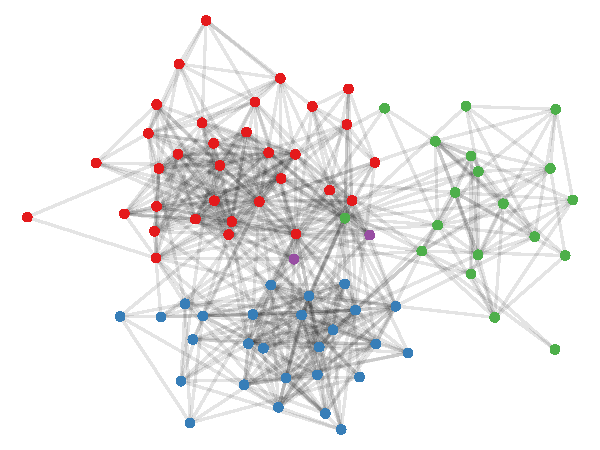
\includegraphics{proposal_files/figure-latex/unnamed-chunk-1-1} 

}

\caption{Points sampled uniformly on two parallel unit length line segments}\label{fig:unnamed-chunk-1}
\end{figure}

We will motivate an approach by the following example.

\begin{example}
Let $U_1, ..., U_n \stackrel{\text{iid}}{\sim}Uniform(0, 1)$ with order statistics 
$U_{(1)}, ..., U_{(n)}$. Then $\forall a \in (0, 1)$ and $\delta \in (0, 1)$, $\exists N = N(\delta, a) < \infty$ such that $\forall n \geq N$, 

\begin{equation}
P(\max_i U_{(i+1)} - U_{(i)} \leq a) \geq 1 - \delta / 2
\end{equation}

Where $N(\delta, a)$ is monotone increasing with respect to $\delta$ and $a$. To prove this, we start with the fact that $U_{(i+1)} - U_{(i)} \sim Beta(1, n)$. Then 

\begin{equation}
P(U_{(i+1)} - U_{(i)} \leq a) = 1 - (1 - a)^n
\end{equation}

and 

\begin{equation}
\label{eq:unsolvable}
P(\max_i U_{(i+1)} - U_{(i)} \leq a) \geq (P(U_{(i+1)} - U_{(i)} \leq a))^n = (1 - (1 - a)^n)^n
\end{equation}

This expression is monotone increasing $\forall n \geq N_1$ for some $N_1 < \infty$. 
Setting $(1 - (1 - a)^{N_2})^{N_2} \geq 1 - \delta / 2$, we can solve for a finite ${N_2}$. Then $N = \max(N_1, N_2)$.
\end{example}

If we extend this example such that \(n_1\) points are sampled uniformly
from the segment \(f_1(t) = (t, 0)\) and \(n_2\) points are sampled
uniformly from the segment \(f_2(t) = (t, a)\) for
\(t \in [0, \cos \frac{\pi}{2} a]\), then a sample of size
\(\min(n_1, n_2) \geq N(\delta, a)\) is sufficient to satisfy:

\begin{equation}
P(\max_i X_{(i+1)} - X_{(i)} \leq a \leq \min_{i, j} \|X_i - Y_j\|) 
\geq 1 - \delta / 2
\end{equation}

and similar for
\(P(\max_j Y_{(j+1)} - Y_{(j)} \leq \min_{i, j} \|X_i - Y_j\|)\), for
\(X_i\) in the first segment and \(Y_j\) in the second segment and
\(X_{(i)}\), \(Y_{(j)}\) are order statistics in the first coordinate.
If each segment corresponds to a community, this leads to the following
two results:

\begin{enumerate}
\def\labelenumi{\arabic{enumi}.}
\item
  Single linkage clustering with \(K = 2\) will perform perfect
  community detection with probability at least \(1 - \delta\).
\item
  An \(\epsilon\)-neighborhood graph with \(\epsilon \in (0, a)\) will
  consists of at least 2 disjoint subgraphs such that no subgraph
  consists of members of two different communities (analogous to the
  SDP), with probability at least \(1 - \delta\).
\end{enumerate}

We can then further extend this to the case where points are drawn from
unit segments with noise. It is straightforward to show that if the
maximum noise is less than \(a / 3\), we can obtain a similar result as
in the noiseless case. Thus if the distribution on the two segments is
used to draw \((A, X) \sim \text{RDPG}(F, n)\), the same properties
should hold for large \(n\).

\hypertarget{manifolds}{%
\subsection{Manifolds}\label{manifolds}}

If instead of sampling uniformly from line segments of unit length, we
sample uniformly from a 1 dimensional manifolds of unit length, the
above property still holds. Let
\(U_1, ..., U_n \stackrel{iid}{\sim} Uniform(0, 1)\) and
\(f : [0, 1] \mapsto \mathbb{R}^d\) be a smooth function such that
\(\int_u^v \sqrt{\sum_k (df_k / dt)^2} dt = \|u - v\|\). Then
\(U_{(i+1)} - U_{(i)} \geq \|f(U_{(i+1)}) - f(U_{(i)})\|\), so
\(P(U_{(i+1)} - U_{(i)} \leq \alpha) \leq P(\|f(U_{(i+1)}) - f(U_{(i)})\| \leq a)\).
If the shortest distance between the two manifolds defined by \(f_1\)
and \(f_2\) with the same restriction is \(a\), then the same \(N\) as
before is sufficient, although perhaps a more lenient lower bound can be
derived based on the shape of \(f_k(\cdot)\).

Our proposed work extends these results by the following.

\begin{enumerate}
\def\labelenumi{\arabic{enumi}.}
\tightlist
\item
  Show that the ASE of a (G)RDPG generated by this type of latent
  configuration produces the correct conditions as described above to
  apply the same probability statements.
\item
  Extend these results by deriving similar probability statements for
  nonuniform distributions.
\item
  Relax the condition for the minimum distance between manifolds by
  investigating alternative clustering techniques on the latent space
  (e.g., spectral clustering).
\end{enumerate}

\hypertarget{summary}{%
\section{Summary}\label{summary}}

For this research, we propose using the connection between Block Models
and the (Generalized) Random Dot Product Graph to motivate community
detection methods. Previous research shows that the Stochastic Block
Model and Degree Corrected Block Model have very structured latent
configurations in the RDPG framework, and these latent structures can be
used to develop community detection algorithms that result in perfect
community detection for large \(n\). In the same vein, we investigated
the connection between the Popularity Adjusted Block Model and the GRDPG
to motivate two community detection algorithms, the first of which is an
application of an existing algorithm, Sparse Subspace Clustering, and
the second is a new algorithm based on the particular latent form of the
PABM, Orthogonal Spectral Clustering. Furthermore, we showed that for
large \(n\), our application of the SSC algorithm to the PABM upholds
the Subspace Detection Property for large yet finite \(n\), and the
output of OSC results in perfect community detection almost surely as
\(n \to \infty\). We will extend these theoretical results with
empirical simulations and real data examples. Finally, we will implement
these two community detection algorithms in an R package.

We aim to extend these results by defining more general structures in
the latent space to construct RDPG or GRDPG models and show that
community detection is possible via Adjacency Spectral Embedding. So
far, we showed that if in the latent space the communities can be
represented as points sampled uniformly on curves or one-dimensional
manifolds separated by a nonzero distance, we can apply two existing
clustering techniques to the ASE and show that they will perform perfect
community detection with high probability. We will generalize these
results to nonuniform distributions on higher dimensional manifolds as
well as investigate alternative clustering techniques for the latent
space that may perform better for smaller \(n\).

\hypertarget{estimated-timeline-of-completion}{%
\subsection{Estimated Timeline of
Completion}\label{estimated-timeline-of-completion}}

Literature review: August 2021

Complete proofs of main theorems: January 2022

Simulations, real data analyses, R package: March 2022

Dissertation completion: April 2022

\renewcommand\refname{References}
  \bibliography{proposal.bib}

\end{document}
